\begin{figure}[h!]
	\centering
	
	
	\tikzset{every picture/.style={line width=0.75pt}} %set default line width to 0.75pt        
	
	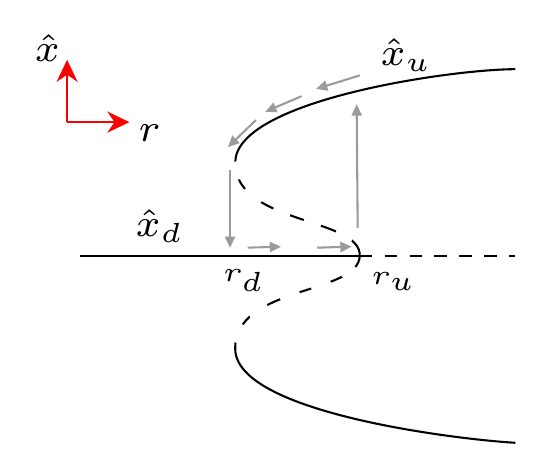
\begin{tikzpicture}[x=0.75pt,y=0.75pt,yscale=-1.5,xscale=1.5]
		%uncomment if require: \path (0,300); %set diagram left start at 0, and has height of 300
		
		%Curve Lines [id:da3475967864092384] 
		\draw    (330,60) .. controls (309.5,60) and (240,70) .. (240,90) .. controls (240,110) and (280.5,107.5) .. (280,120) .. controls (279.5,132.5) and (239.5,129.5) .. (240,150) .. controls (240.5,170.5) and (312,179) .. (330,180) ;
		%Straight Lines [id:da8628159498522963] 
		\draw    (190,120) -- (280,120) ;
		%Straight Lines [id:da07087007695378178] 
		\draw  [dash pattern={on 4.5pt off 4.5pt}]  (280,120) -- (330,120) ;
		%Straight Lines [id:da9630925968212913] 
		\draw [color={rgb, 255:red, 255; green, 255; blue, 255 }  ,draw opacity=1 ][line width=3]    (240,89.67) -- (241.33,95.33) ;
		%Straight Lines [id:da10933997251577554] 
		\draw [color={rgb, 255:red, 255; green, 255; blue, 255 }  ,draw opacity=1 ][line width=3]    (243.33,98.33) -- (248,103) ;
		%Straight Lines [id:da39451280789014165] 
		\draw [color={rgb, 255:red, 255; green, 255; blue, 255 }  ,draw opacity=1 ][line width=3]    (252.33,104.67) -- (257.67,106.67) ;
		%Straight Lines [id:da7877273412409396] 
		\draw [color={rgb, 255:red, 255; green, 255; blue, 255 }  ,draw opacity=1 ][line width=3]    (262,108.67) -- (267.33,110.67) ;
		%Straight Lines [id:da949863006732423] 
		\draw [color={rgb, 255:red, 255; green, 255; blue, 255 }  ,draw opacity=1 ][line width=3]    (272.33,112.33) -- (277.67,114.33) ;
		%Straight Lines [id:da6008132146686285] 
		\draw [color={rgb, 255:red, 255; green, 255; blue, 255 }  ,draw opacity=1 ][line width=3]    (275,127.33) -- (278.67,123.67) ;
		%Straight Lines [id:da6428214676220647] 
		\draw [color={rgb, 255:red, 255; green, 255; blue, 255 }  ,draw opacity=1 ][line width=3]    (264.67,131) -- (270.67,128.33) ;
		%Straight Lines [id:da557059542843994] 
		\draw [color={rgb, 255:red, 255; green, 255; blue, 255 }  ,draw opacity=1 ][line width=3]    (254.67,134.33) -- (260.67,131.67) ;
		%Straight Lines [id:da14327656158346214] 
		\draw [color={rgb, 255:red, 255; green, 255; blue, 255 }  ,draw opacity=1 ][line width=3]    (244.33,138.67) -- (250.33,136) ;
		%Straight Lines [id:da5660831756940781] 
		\draw [color={rgb, 255:red, 255; green, 255; blue, 255 }  ,draw opacity=1 ][line width=3]    (239.33,147.33) -- (242.33,142) ;
		%Straight Lines [id:da3939017840273582] 
		\draw [color={rgb, 255:red, 255; green, 0; blue, 0 }  ,draw opacity=1 ]   (186,77) -- (203,77) ;
		\draw [shift={(206,77)}, rotate = 180] [fill={rgb, 255:red, 255; green, 0; blue, 0 }  ,fill opacity=1 ][line width=0.08]  [draw opacity=0] (7.14,-3.43) -- (0,0) -- (7.14,3.43) -- (4.74,0) -- cycle    ;
		%Straight Lines [id:da4292502511319951] 
		\draw [color={rgb, 255:red, 255; green, 0; blue, 0 }  ,draw opacity=1 ]   (186,77) -- (186,60) ;
		\draw [shift={(186,57)}, rotate = 90] [fill={rgb, 255:red, 255; green, 0; blue, 0 }  ,fill opacity=1 ][line width=0.08]  [draw opacity=0] (7.14,-3.43) -- (0,0) -- (7.14,3.43) -- (4.74,0) -- cycle    ;
		%Straight Lines [id:da04468453728060462] 
		\draw [color={rgb, 255:red, 155; green, 155; blue, 155 }  ,draw opacity=1 ]   (268.87,65.45) -- (280,62) ;
		\draw [shift={(266,66.33)}, rotate = 342.8] [fill={rgb, 255:red, 155; green, 155; blue, 155 }  ,fill opacity=1 ][line width=0.08]  [draw opacity=0] (3.57,-1.72) -- (0,0) -- (3.57,1.72) -- cycle    ;
		%Straight Lines [id:da6421999189293346] 
		\draw [color={rgb, 255:red, 155; green, 155; blue, 155 }  ,draw opacity=1 ]   (252.42,72.48) -- (261.33,68.67) ;
		\draw [shift={(249.67,73.67)}, rotate = 336.8] [fill={rgb, 255:red, 155; green, 155; blue, 155 }  ,fill opacity=1 ][line width=0.08]  [draw opacity=0] (3.57,-1.72) -- (0,0) -- (3.57,1.72) -- cycle    ;
		%Straight Lines [id:da3913600379521629] 
		\draw [color={rgb, 255:red, 155; green, 155; blue, 155 }  ,draw opacity=1 ]   (239.83,82.92) -- (246.67,76.33) ;
		\draw [shift={(237.67,85)}, rotate = 316.08] [fill={rgb, 255:red, 155; green, 155; blue, 155 }  ,fill opacity=1 ][line width=0.08]  [draw opacity=0] (3.57,-1.72) -- (0,0) -- (3.57,1.72) -- cycle    ;
		%Straight Lines [id:da2959398371731523] 
		\draw [color={rgb, 255:red, 155; green, 155; blue, 155 }  ,draw opacity=1 ]   (238.33,114.33) -- (238.33,92.33) ;
		\draw [shift={(238.33,117.33)}, rotate = 270] [fill={rgb, 255:red, 155; green, 155; blue, 155 }  ,fill opacity=1 ][line width=0.08]  [draw opacity=0] (3.57,-1.72) -- (0,0) -- (3.57,1.72) -- cycle    ;
		%Straight Lines [id:da6212681777845439] 
		\draw [color={rgb, 255:red, 155; green, 155; blue, 155 }  ,draw opacity=1 ]   (251.67,117.09) -- (244,117.33) ;
		\draw [shift={(254.67,117)}, rotate = 178.21] [fill={rgb, 255:red, 155; green, 155; blue, 155 }  ,fill opacity=1 ][line width=0.08]  [draw opacity=0] (3.57,-1.72) -- (0,0) -- (3.57,1.72) -- cycle    ;
		%Straight Lines [id:da8168119094171771] 
		\draw [color={rgb, 255:red, 155; green, 155; blue, 155 }  ,draw opacity=1 ]   (274.33,117.09) -- (266.33,117.33) ;
		\draw [shift={(277.33,117)}, rotate = 178.26] [fill={rgb, 255:red, 155; green, 155; blue, 155 }  ,fill opacity=1 ][line width=0.08]  [draw opacity=0] (3.57,-1.72) -- (0,0) -- (3.57,1.72) -- cycle    ;
		%Straight Lines [id:da604904148477025] 
		\draw [color={rgb, 255:red, 155; green, 155; blue, 155 }  ,draw opacity=1 ]   (279.03,74.33) -- (279.33,111) ;
		\draw [shift={(279,71.33)}, rotate = 89.52] [fill={rgb, 255:red, 155; green, 155; blue, 155 }  ,fill opacity=1 ][line width=0.08]  [draw opacity=0] (3.57,-1.72) -- (0,0) -- (3.57,1.72) -- cycle    ;
		
		% Text Node
		\draw (207,76) node [anchor=north west][inner sep=0.75pt]  [font=\scriptsize,xscale=2,yscale=2] [align=left] {$\displaystyle r$};
		% Text Node
		\draw (173.67,47) node [anchor=north west][inner sep=0.75pt]  [font=\scriptsize,xscale=2,yscale=2] [align=left] {$\displaystyle \hat{x}$};
		% Text Node
		\draw (234,122.33) node [anchor=north west][inner sep=0.75pt]  [font=\tiny,xscale=2,yscale=2] [align=left] {$\displaystyle r_{d}$};
		% Text Node
		\draw (281.67,123.33) node [anchor=north west][inner sep=0.75pt]  [font=\tiny,xscale=2,yscale=2] [align=left] {$\displaystyle r_{u}$};
		% Text Node
		\draw (206,103) node [anchor=north west][inner sep=0.75pt]  [font=\scriptsize,xscale=2,yscale=2] [align=left] {$\displaystyle \hat{x}_{d}$};
		% Text Node
		\draw (284.67,48.33) node [anchor=north west][inner sep=0.75pt]  [font=\scriptsize,xscale=2,yscale=2] [align=left] {$\displaystyle \hat{x}_{u}$};
		
		
	\end{tikzpicture}
\end{figure}